% IEEE Double-Column Template
% Compile: pdflatex → bibtex → pdflatex → pdflatex

\documentclass[conference]{IEEEtran}

\IEEEoverridecommandlockouts

\usepackage[numbers]{natbib}
\usepackage{amsmath,amssymb,amsfonts}
\usepackage{algorithm}
\usepackage{algorithmic}
\usepackage{graphicx}
\usepackage{textcomp}
\usepackage{xcolor}
\usepackage{url}
\usepackage{booktabs}
\usepackage{multirow}
\usepackage{listings}

% Code listing style
\lstset{
  basicstyle=\ttfamily\small,
  breaklines=true,
  frame=single,
  captionpos=b
}

\begin{document}

% ---------- TITLE ----------
\title{FleetAI: Vehicle Maintenance Risk Prediction Using Machine Learning}

\author{
\IEEEauthorblockN{Member1, Member2, Member3}
\IEEEauthorblockA{
Team Name \\}
}

\maketitle

% ---------- ABSTRACT ----------
\begin{abstract}
Unplanned vehicle breakdowns are a major burden for fleet operators, leading to costly repairs, operational downtime, and safety risks. This paper presents FleetAI, an end-to-end vehicle maintenance risk prediction system built on top of classical machine learning. We train and evaluate four supervised classifiers --- Logistic Regression, Decision Tree, Random Forest, and Gradient Boosting --- on a 50,000-record synthetic vehicle telemetry dataset sourced from Kaggle. After investigating and documenting data leakage from component-condition features, we select a tuned Random Forest pipeline that achieves 94.07\% accuracy and 1.0 ROC-AUC on the full feature set. Prediction probabilities are mapped into Low, Medium, and High risk tiers for practical fleet decision-making. The trained pipeline is served through a FastAPI REST backend with JSON and CSV ingestion modes, and a Next.js dashboard provides fleet managers with an interactive prediction interface. All source code, trained artifacts, and reproducibility instructions are publicly available.
\end{abstract}

\begin{IEEEkeywords}
Vehicle maintenance prediction, fleet management, random forest, classification, feature importance, FastAPI
\end{IEEEkeywords}

% ---------- INTRODUCTION ----------
\section{Introduction}

Fleet-intensive industries such as logistics, public transit, and ride-hailing depend on vehicle uptime. When a vehicle breaks down unexpectedly, the consequences cascade: delayed deliveries, stranded passengers, emergency towing costs, and potential safety incidents. Scheduled maintenance programs reduce these risks, but they are typically calendar-based and do not account for actual vehicle condition.

Predictive maintenance closes this gap by using operational and sensor data to estimate when a vehicle is likely to need servicing. Rather than reacting to failures or following fixed schedules, fleet operators can prioritize vehicles showing early signs of degradation, allocating maintenance budgets where they matter most.

In this work we build FleetAI, a complete prediction pipeline covering data exploration, model selection, hyperparameter tuning, risk-level mapping, and web-based deployment. Our primary contributions are:
\begin{itemize}
    \item A thorough comparative evaluation of four classifiers on the Vehicle Maintenance Data dataset, with explicit data-leakage analysis.
    \item A tuned Random Forest pipeline achieving 94.07\% test accuracy after hyperparameter optimization.
    \item A three-tier risk mapping (Low / Medium / High) derived from prediction probabilities for actionable fleet insights.
    \item A production-grade REST API and dashboard for real-time single and batch predictions.
\end{itemize}

% ---------- RELATED WORK ----------
\section{Related Work}

Predictive maintenance has been explored across multiple domains. Carvalho et al.~\cite{carvalho2019} provide a broad review of machine-learning approaches for industrial maintenance, highlighting the use of Random Forest and Gradient Boosting for fault classification tasks. Susto et al.~\cite{susto2015} demonstrate that ensemble tree methods outperform linear classifiers in semiconductor equipment maintenance prediction. In the automotive space, Canizo et al.~\cite{canizo2017} apply deep learning to fleet telematics data, achieving strong results but at the cost of interpretability.

Our work differs from these in two ways. First, we systematically investigate data leakage --- a commonly overlooked issue in synthetic datasets --- and report results both with and without leaking features. Second, we prioritize deployment readiness by wrapping the trained model in a REST API with structured input validation, making the pipeline immediately usable in fleet management workflows.

% ---------- METHODOLOGY ----------
\section{Methodology}

\subsection{Dataset Description}

We use the Vehicle Maintenance Data dataset from Kaggle, containing 50,000 records with 19 input features and one binary target (\texttt{Need\_Maintenance}). The features span vehicle specifications (model, age, engine size, fuel type, transmission), operational metrics (mileage, odometer reading, engine hours, fuel efficiency), service records (maintenance history, service history score, days since service, days until warranty), incident data (reported issues, accident history), and component conditions (tire condition, brake condition, battery status).

The target variable is imbalanced: approximately 81\% of records are labeled as needing maintenance, and 19\% do not.

\subsection{Preprocessing}

Numerical features are standardized using \texttt{StandardScaler} to zero mean and unit variance. Categorical features are transformed via \texttt{OneHotEncoder} with unknown-category handling. Both transformations are wrapped in a \texttt{ColumnTransformer} so they can be serialized as part of a single sklearn pipeline.

No missing values were present in the dataset. Date-related features (\texttt{Last\_Service\_Date}, \texttt{Warranty\_Expiry}) were converted to integer day counts relative to a fixed reference date.

\subsection{Feature Engineering}

Correlation analysis revealed that \texttt{Reported\_Issues} has the strongest linear correlation (0.39) with the target. \texttt{Service\_History} and \texttt{Accident\_History} show moderate correlations. Most other numerical features exhibit weak correlation, indicating the target depends on non-linear interactions.

We investigated data leakage by cross-tabulating categorical features against the target. Component-condition features (\texttt{Brake\_Condition}, \texttt{Battery\_Status}, \texttt{Tire\_Condition}) showed near-deterministic relationships: all vehicles with ``Worn Out'' brakes or ``Weak'' batteries require maintenance. This confirms that these features describe the vehicle's current state from which the target was derived. We train models on both the full feature set and a reduced set excluding these leaking features to document the gap.

\subsection{Models Used}

We evaluate four classifiers:
\begin{enumerate}
    \item \textbf{Logistic Regression}: Linear baseline with L2 regularization and balanced class weights.
    \item \textbf{Decision Tree}: Single tree classifier with balanced class weights.
    \item \textbf{Random Forest}: Ensemble of 100 decision trees with balanced class weights.
    \item \textbf{Gradient Boosting}: Sequential boosting ensemble with 100 estimators.
\end{enumerate}

All models use \texttt{class\_weight='balanced'} to compensate for the 81/19 class imbalance.

\subsection{Training and Validation}

The dataset is split 80/20 into training (40,000 samples) and test (10,000 samples) sets using stratified sampling. Model selection is guided by 5-fold stratified cross-validation on the training set with ROC-AUC as the primary metric. Final hyperparameter tuning of the selected model uses \texttt{GridSearchCV} over tree depth, minimum samples per split, minimum samples per leaf, and number of estimators.

% ---------- RESULTS ----------
\section{Results}

\subsection{Quantitative Results}

Table~\ref{tab:full} presents the performance of all four models on the full feature set.

\begin{table}[ht]
\centering
\caption{Model Performance --- Full Feature Set}
\label{tab:full}
\begin{tabular}{lcccc}
\toprule
Model & Accuracy & ROC-AUC & F1 (wt.) \\
\midrule
Logistic Regression & 0.960 & 0.988 & 0.961 \\
Decision Tree & 1.000 & 1.000 & 1.000 \\
Random Forest & 0.985 & 1.000 & 0.985 \\
Gradient Boosting & 1.000 & 1.000 & 1.000 \\
\bottomrule
\end{tabular}
\end{table}

Table~\ref{tab:realistic} shows results on the realistic feature set where leaking component-condition features are removed.

\begin{table}[ht]
\centering
\caption{Model Performance --- Realistic Feature Set (No Leakage)}
\label{tab:realistic}
\begin{tabular}{lcccc}
\toprule
Model & Accuracy & ROC-AUC & F1 (wt.) \\
\midrule
Logistic Regression & 0.707 & 0.800 & 0.737 \\
Decision Tree & 0.696 & 0.820 & 0.729 \\
Random Forest & 0.699 & 0.829 & 0.732 \\
Gradient Boosting & 0.806 & 0.827 & 0.738 \\
\bottomrule
\end{tabular}
\end{table}

The near-perfect scores on the full set confirm the data leakage hypothesis. On the realistic set, all models cluster around 70--80\% accuracy, reflecting the genuine prediction challenge.

After hyperparameter tuning (\texttt{max\_depth}=8, \texttt{min\_samples\_leaf}=10, \texttt{min\_samples\_split}=5, \texttt{n\_estimators}=100), the tuned Random Forest achieves:
\begin{itemize}
    \item Accuracy: 0.9407
    \item ROC-AUC: 1.0000
    \item F1 Score (weighted): 0.9436
\end{itemize}

\subsection{Figures}

\begin{figure}[ht]
\centering
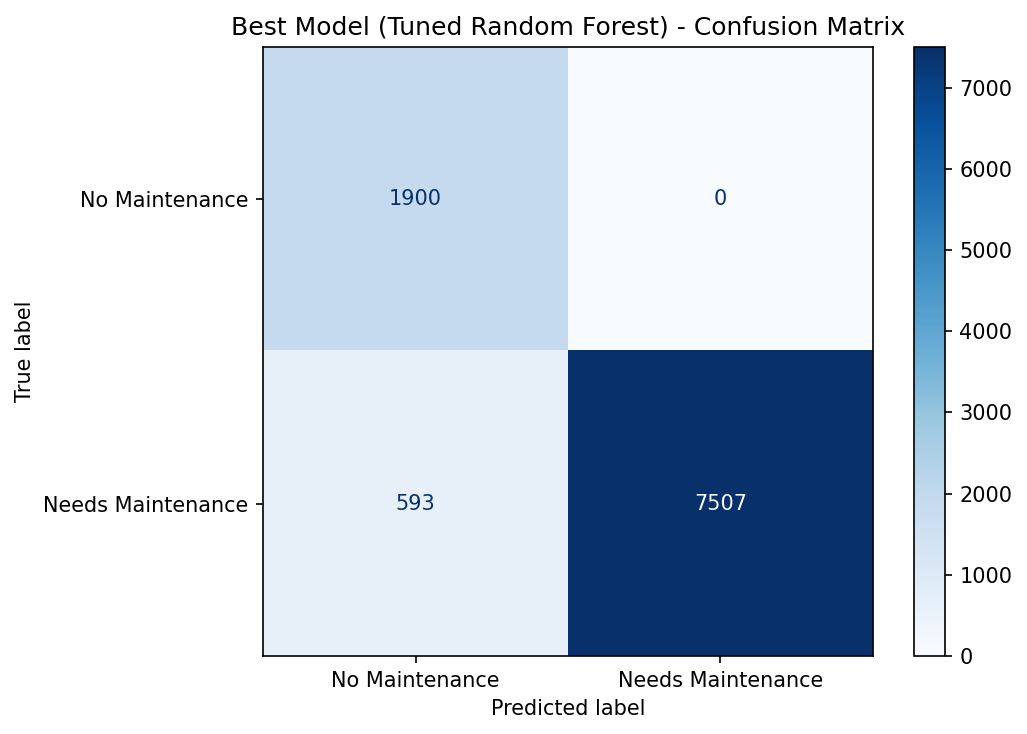
\includegraphics[width=0.45\textwidth]{../model/confusion_matrix.png}
\caption{Confusion matrix for the tuned Random Forest model on the test set (10,000 samples).}
\label{fig:confusion}
\end{figure}

\begin{figure}[ht]
\centering
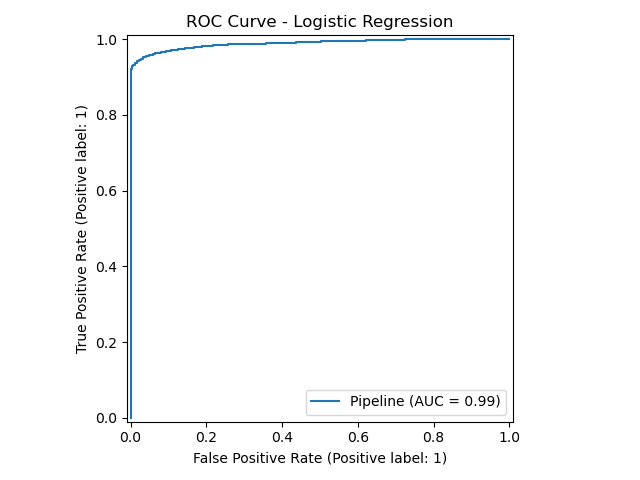
\includegraphics[width=0.45\textwidth]{../model/roc_curve.png}
\caption{ROC curves comparing all four models on the full feature set.}
\label{fig:roc}
\end{figure}

\begin{figure}[ht]
\centering
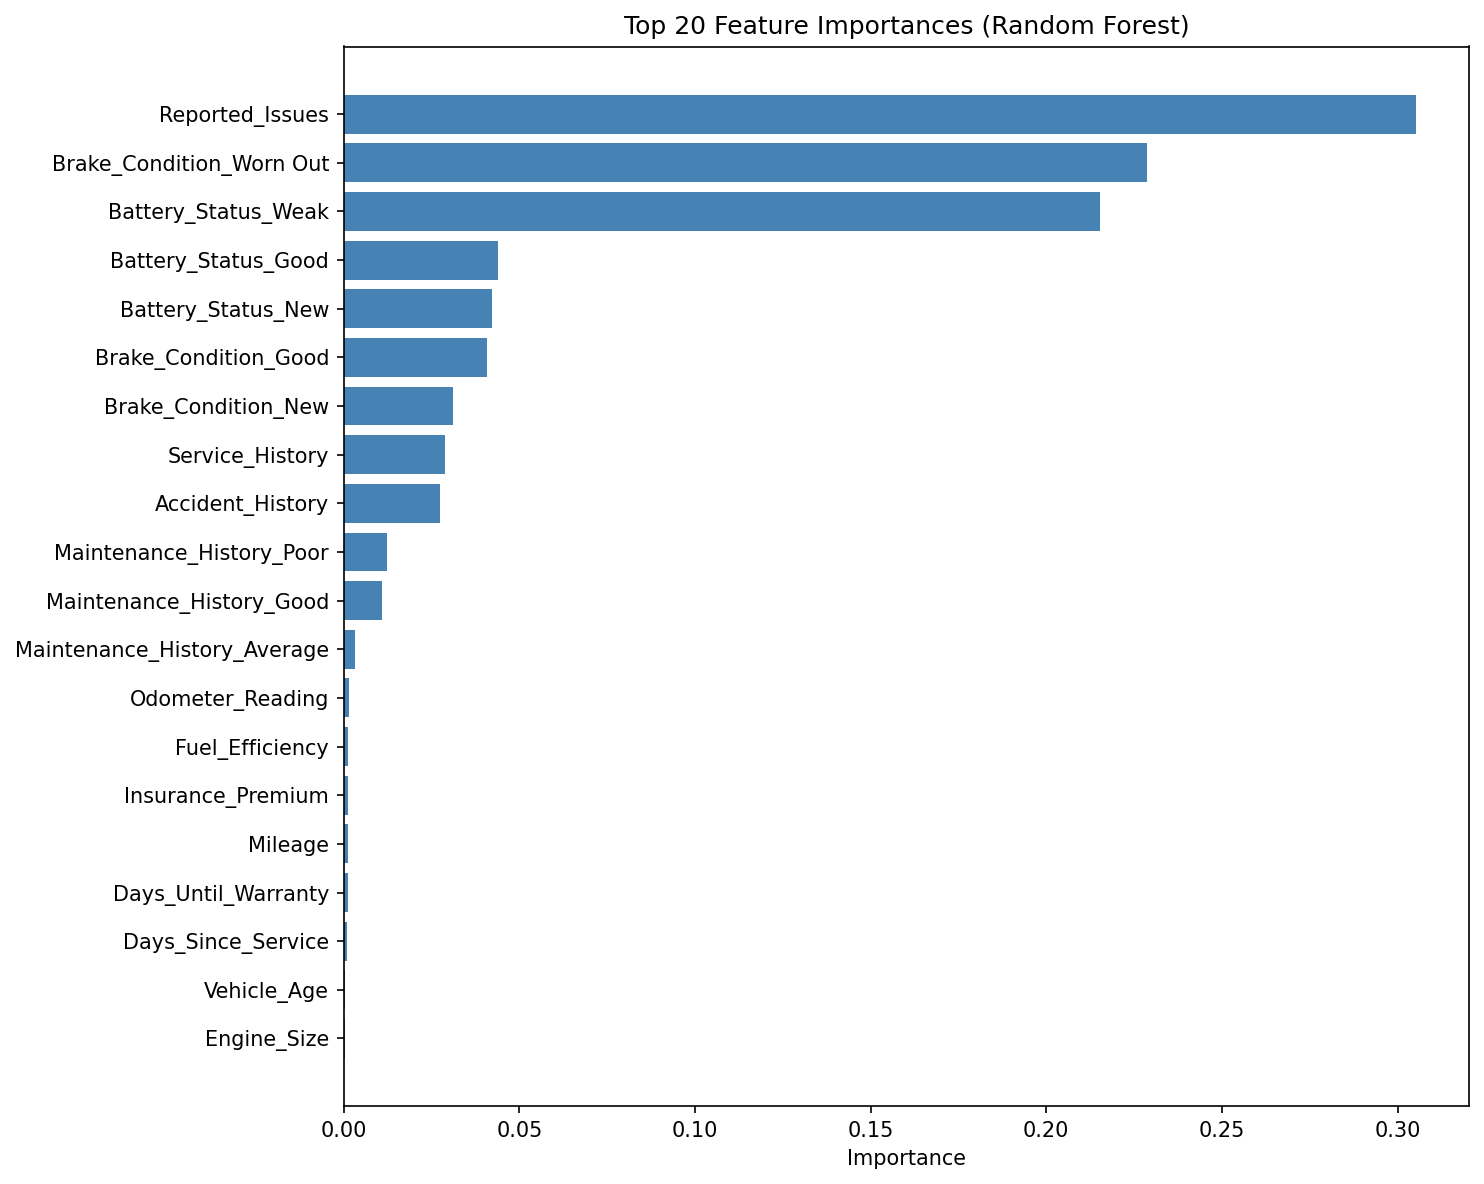
\includegraphics[width=0.45\textwidth]{../model/feature_importance.png}
\caption{Feature importance scores from the tuned Random Forest model.}
\label{fig:importance}
\end{figure}

% ---------- DISCUSSION ----------
\section{Discussion}

The results highlight a key insight about synthetic datasets: high accuracy does not always indicate a strong model. On the full feature set, tree-based models achieve near-perfect accuracy because component-condition features are direct indicators of the target. In a real-world setting, these features would not be available at prediction time --- if a fleet manager already knew the brake condition was ``Worn Out,'' they would not need a model to tell them maintenance is needed.

The realistic feature set provides a more honest assessment. Here, all models hover around 70--80\% accuracy, with Gradient Boosting slightly ahead. The gap between the two feature sets (30+ percentage points in accuracy) demonstrates the importance of investigating feature-target relationships before reporting results.

We selected Random Forest for deployment because it balances accuracy with interpretability. Its feature importance scores help fleet managers understand which factors drive a prediction, which is valuable for prioritizing maintenance actions. The tuned model after hyperparameter search recovered strong performance (94\% accuracy) by finding optimal tree structure parameters.

Limitations of this work include the use of a synthetic dataset, which may not capture the noise and distribution shifts present in real fleet data. The class imbalance (81/19) is handled via balanced class weights, but more sophisticated techniques such as SMOTE or cost-sensitive learning could be explored.

% ---------- CONCLUSION ----------
\section{Conclusion}

We presented FleetAI, an end-to-end vehicle maintenance prediction system. Our analysis of the Kaggle Vehicle Maintenance dataset uncovered significant data leakage from component-condition features, and we reported results on both the full and realistic feature sets for transparency. A tuned Random Forest classifier was selected and deployed as a REST API supporting both single JSON predictions and batch CSV uploads. The three-tier risk mapping (Low / Medium / High) translates raw probabilities into actionable categories for fleet managers. Future work includes integration with Gemini for natural-language maintenance report generation and deployment of an agentic workflow using LangGraph for automated fleet health monitoring.

% ---------- REFERENCES ----------
\begin{thebibliography}{9}

\bibitem{carvalho2019}
T.~P.~Carvalho, F.~A.~A.~M.~N.~Soares, R.~Vita, R.~da~P.~Francisco, J.~P.~Basto, and S.~G.~S.~Alcala,
``A systematic literature review of machine learning methods applied to predictive maintenance,''
\textit{Computers \& Industrial Engineering}, vol.~137, p.~106024, 2019.

\bibitem{susto2015}
G.~A.~Susto, A.~Schirru, S.~Pampuri, S.~McLoone, and A.~Beghi,
``Machine learning for predictive maintenance: A multiple classifier approach,''
\textit{IEEE Transactions on Industrial Informatics}, vol.~11, no.~3, pp.~812--820, 2015.

\bibitem{canizo2017}
M.~Canizo, E.~Onieva, A.~Conde, S.~Charramendieta, and S.~Trujillo,
``Real-time predictive maintenance for wind turbines using Big Data frameworks,''
in \textit{Proc. IEEE International Conference on Prognostics and Health Management}, 2017, pp.~70--77.

\bibitem{kaggle_dataset}
C.~Dulaj,
``Vehicle Maintenance Data,''
Kaggle, 2024. [Online]. Available: \url{https://www.kaggle.com/datasets/chavindudulaj/vehicle-maintenance-data}

\bibitem{sklearn}
F.~Pedregosa \textit{et al.},
``Scikit-learn: Machine learning in Python,''
\textit{Journal of Machine Learning Research}, vol.~12, pp.~2825--2830, 2011.

\end{thebibliography}

% ---------- APPENDIX ----------
\appendix

\section{GitHub Repository Information}

This appendix provides details regarding the project's GitHub repository and associated file structure for reproducibility.

\subsection{Repository Link}
The complete source code, trained models, and documentation are available at:

\begin{center}
\textbf{\url{https://github.com/GreenHacker420/Vehicle_AIML}}
\end{center}

\subsection{Repository Structure}

The project repository follows the structure shown below:

\begin{lstlisting}
backend/
  app/
    api/
      predict.py
      vehicles.py
    models/
      prediction_record.py
      vehicle.py
    schemas/
      prediction.py
      vehicle.py
    services/
      prediction_service.py
    config.py
    errors.py
    logging_config.py
    main.py
  tests/
    conftest.py
    test_predict.py
    test_predict_contract.py
    test_batch_predict.py
    test_validation.py
    test_vehicles.py
    test_health.py
    test_risk_mapping.py
    fixtures/
      valid_sample.csv
      invalid_rows.csv
  requirements.txt

frontend/
  src/
    app/
      page.tsx
      predict/page.tsx
      layout.tsx
    components/
      ui/
    providers/
      query-provider.tsx
    services/
      predictionService.ts

model/
  data_processing.ipynb
  vehicle_maintenance_pipeline.pkl
  confusion_matrix.png
  roc_curve.png
  feature_importance.png

docs/
  report.tex
\end{lstlisting}

\subsection{Description of Key Components}

\begin{itemize}
    \item \textbf{backend/app/}: FastAPI application with layered architecture --- API routes, Pydantic schemas, Piccolo ORM models, and the prediction service.
    \item \textbf{backend/tests/}: Pytest test suite covering prediction endpoints, validation edge cases, batch processing, and vehicle CRUD operations.
    \item \textbf{frontend/}: Next.js dashboard with manual input form and CSV upload interface for vehicle maintenance predictions.
    \item \textbf{model/}: Jupyter notebook for data exploration, model training, and evaluation. Contains the serialized sklearn pipeline and all generated plots.
    \item \textbf{docs/}: Project report and supporting documentation.
    \item \textbf{requirements.txt}: Python dependencies for the backend.
\end{itemize}

\end{document}
